\section{Introduction}\label{introduction}

\frame{\tableofcontents[hidesubsections]}

\begin{frame}{Introduction - 自我介绍}

\begin{itemize}
\itemsep1pt\parskip0pt\parsep0pt
\item
  American pediatrician - 美国儿科医生
\item
  Lived in China for 22 years - 在中国生活22年
\item
  Married for 28 years (prettiest surgeon in Northwest China!) -
  结婚28年(中国西北最美的外科医生)
\item
  Two daughters (23 and 17 years old) - 有两个女儿(一个23岁,一个17岁)
\end{itemize}

\end{frame}

\begin{frame}{Family - 家庭}

\begin{figure}
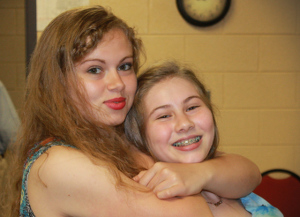
\includegraphics[scale=0.7]{./img/img_0002_300.jpg}
\end{figure}

\end{frame}

\section{Problem}\label{problem}

\subsection{Cervical Cancer}\label{cervical-cancer}

\begin{frame}{Cervical cancer in rural Muslim women}

\begin{itemize}
\itemsep1pt\parskip0pt\parsep0pt
\item
  Local partners and their patients
\item
  Patient ignorance
\item
  Local partner ignorance
\item
  Local hospital's spotty care
\end{itemize}

\end{frame}

\section{Investigation}\label{investigation}

\subsection{What is the current
situation?}\label{what-is-the-current-situation}

\begin{frame}{Asking around - someone knows this stuff!}

\begin{itemize}
\itemsep1pt\parskip0pt\parsep0pt
\item
  Pap smears are available
\item
  Thin prep analysis of pap smears is available
\item
  Treatment for early stage cervical cancer is available
\end{itemize}

\end{frame}

\subsection{Why is it that way?}\label{why-is-it-that-way}

\begin{frame}{Asking ``Why?''}

\begin{itemize}
\itemsep1pt\parskip0pt\parsep0pt
\item
  Hezheng county
\item
  Linxia county
\item
  Ji Shi Shan county
\end{itemize}

\end{frame}

\section{Resources and Solution}\label{resources-and-solution}

\subsection{Resources}\label{resources}

\begin{frame}{Resources in hand}

\begin{itemize}
\itemsep1pt\parskip0pt\parsep0pt
\item
  Community Health Educators

  \begin{itemize}
  \itemsep1pt\parskip0pt\parsep0pt
  \item
    Local trainer with interest in Muslims and knowledge of the area
  \end{itemize}
\item
  OB/GYN volunteers
\item
  One general/vascular surgeon, one pediatric nephrologist
\end{itemize}

\end{frame}

\begin{frame}{Resources needed}

\begin{itemize}
\itemsep1pt\parskip0pt\parsep0pt
\item
  Expertise
\item
  Money
\item
  Follow up personnel
\end{itemize}

\end{frame}

\subsection{Solution}\label{solution}

\begin{frame}{Kickoff events}

\begin{itemize}
\itemsep1pt\parskip0pt\parsep0pt
\item
  Monthly events alternating sites
\item
  Teaching on cervical cancer - what it is, what it can do, how to
  prevent it
\item
  Pap smears for all women that go through the teaching
\end{itemize}

\end{frame}

\begin{frame}{Follow-up}

\begin{itemize}
\itemsep1pt\parskip0pt\parsep0pt
\item
  Local volunteers
\item
  Take pap smear report back to women, ideally during home visit
\item
  Patients not seen by volunteers followed up with default system
\end{itemize}

\end{frame}

\begin{frame}{Follow-up teams}

\begin{figure}
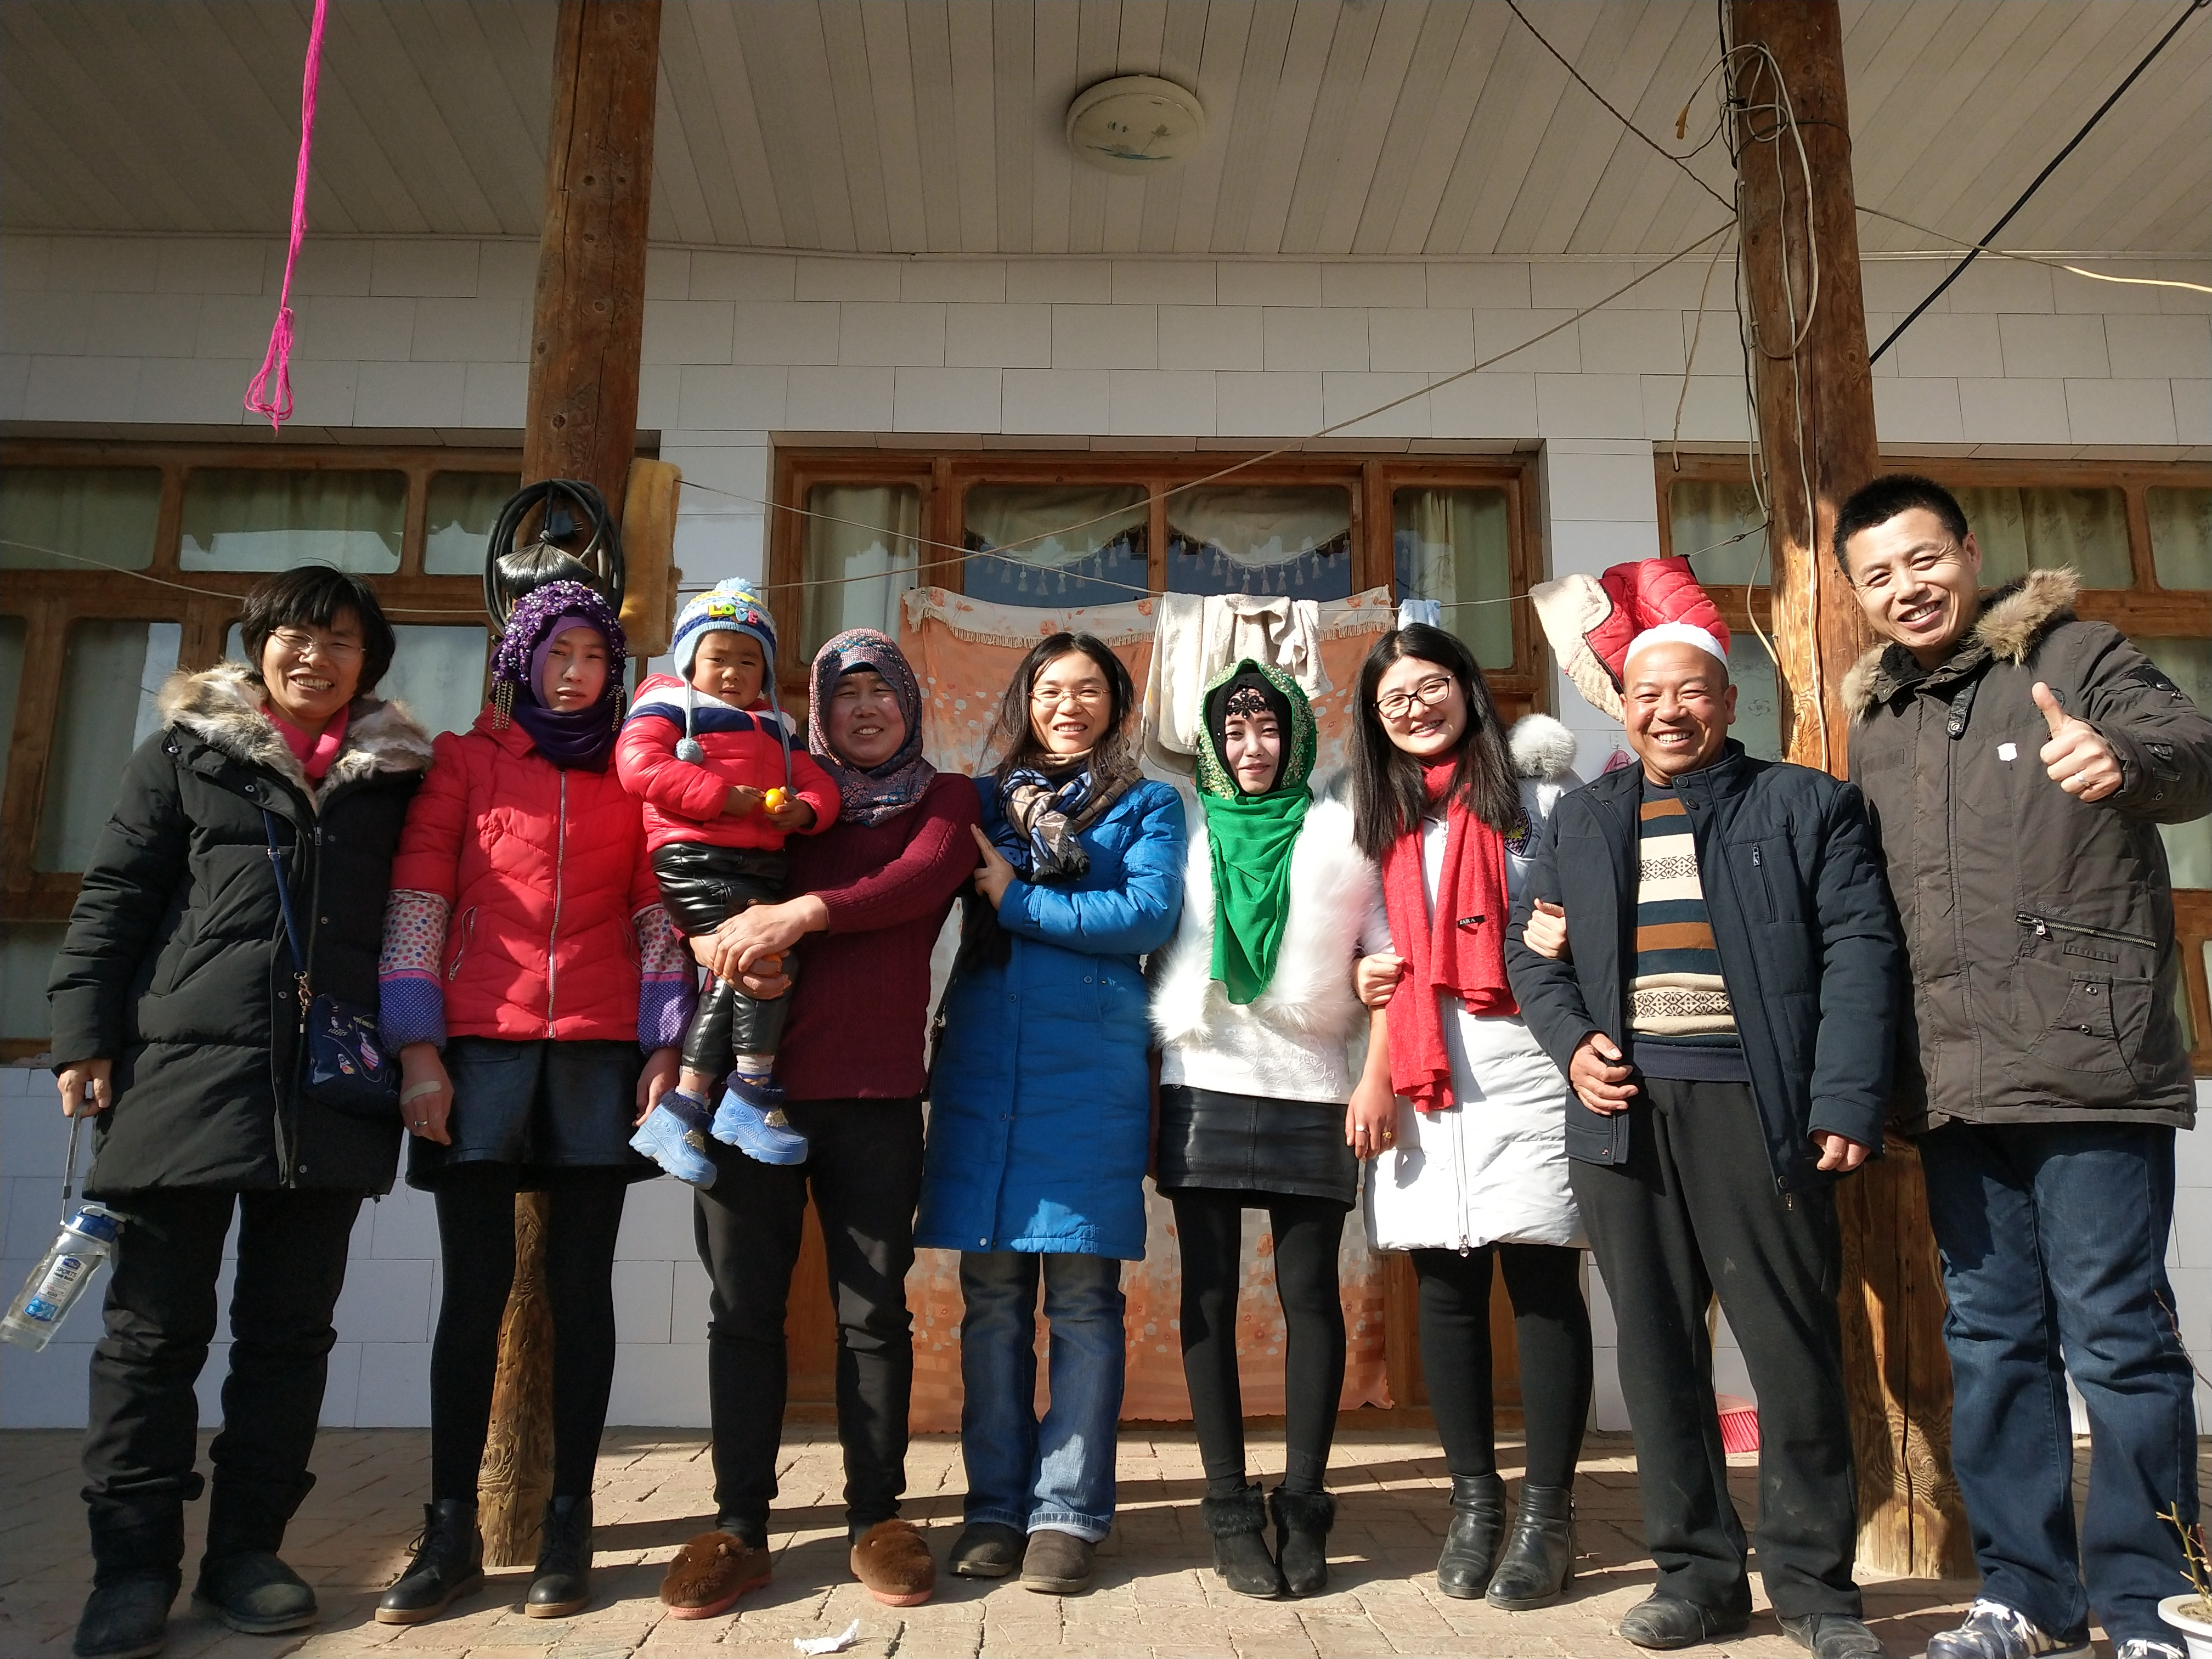
\includegraphics[scale=0.05]{./img/JSS_Followup_300.jpg}
\caption{北京人在积石山}
\end{figure}

\end{frame}

\begin{frame}{2018 Summer plans}

\begin{itemize}
\itemsep1pt\parskip0pt\parsep0pt
\item
  Two follow up teams scheduled
\item
  Multiple interns
\item
  Multiple local cross cultural workers helping
\end{itemize}

\end{frame}

\section{Results and Limitations}\label{results-and-limitations}

\subsection{Results}\label{results}

\begin{frame}{Numerical Results}

\begin{table}
\begin{tabular}{l | l}
Total Number Seen & 303\\
Total Number Screened & 267\\
Percent screened needing intervention & 11.61\% \\
Percent Seen needing intervention & 10.23\% \\
\end{tabular}
\caption{2018 - Numbers so far}
\end{table}

\end{frame}

\begin{frame}{Linxia}

After about 8 months of our screening, Linxia city enacted a city wide
project to screen all women.

\end{frame}

\begin{frame}{Ji Shi Shan}

\begin{itemize}
\itemsep1pt\parskip0pt\parsep0pt
\item
  Open door to continued screening and follow up
\item
  Preparing to do colposcopy training in the summer/fall
\end{itemize}

\end{frame}

\subsection{Limitations}\label{limitations}

\begin{frame}{Limitations}

\begin{itemize}
\itemsep1pt\parskip0pt\parsep0pt
\item
  No pre-program numbers
\item
  Tied to local institutions for teaching and testing
\item
  No HPV vaccine available
\item
  Limited colposcopy available
\end{itemize}

\end{frame}

\section{Questions?}\label{questions}

\begin{frame}{Questions? 提问题?}

\begin{figure}[htbp]
\centering
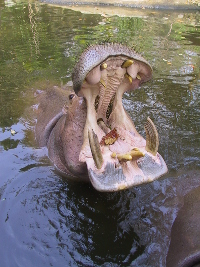
\includegraphics{./img/img_0510_200.jpg}
\caption{}
\end{figure}

\end{frame}
